\documentclass{beamer}
\usepackage{graphicx}
\usepackage{xcolor}
\usepackage{tikz}
\usepackage{amsmath}
\DeclareGraphicsExtensions{.png,.pdf,.jpg,.jpeg}

\definecolor{purpleblue}{RGB}{80, 80, 180}
\definecolor{lightgray}{RGB}{230, 230, 230}
\definecolor{novelPurple}{RGB}{98, 54, 255}
\definecolor{darkgray}{RGB}{50, 50, 50}
\definecolor{softPurple}{RGB}{180, 170, 255}
\definecolor{softGray}{RGB}{235, 235, 245}
\definecolor{lightText}{RGB}{90, 90, 110}
\graphicspath{{static/unit4/}{./}}

\usetheme{Madrid}
\usecolortheme{dolphin}

\setbeamerfont{title}{size=\Large,series=\bfseries}
\setbeamerfont{frametitle}{size=\LARGE,series=\bfseries}
\setbeamercolor{frametitle}{fg=white, bg=novelPurple}
\setbeamercolor{title}{fg=white, bg=purpleblue}

\title[SAT Unit 4.4]{\textbf{SAT Unit 4.4 \\Circles}}
\author{\textbf{Jack Zeng}}
\institute{\textcolor{white}{\textbf{Novel Prep}}}
\date{\today}

\begin{document}

\begin{frame}
    \titlepage
    \vfill
    \begin{flushright}
        \textcolor{purpleblue}{\Huge \textbf{Novel Prep}}
    \end{flushright}
\end{frame}

\begin{frame}
    \begin{tikzpicture}[remember picture, overlay]
        \shade[top color=softPurple, bottom color=softGray]
            (current page.north west) rectangle (current page.south east);
        \fill[white, opacity=0.3] (current page.center) circle (4cm);
        \node[align=center] at (current page.center) {
            {\Huge\bfseries\textcolor{purpleblue}{Novel Prep}} \\[0.5cm]
            {\Large\itshape\textcolor{lightText}{Excellence in SAT Prep}}
        };
        \foreach \x in {1,2,3,4,5} {
            \fill[purpleblue, opacity=0.2] (rand*10-5, rand*7-3.5) circle (0.1+\x*0.05);
        }
    \end{tikzpicture}
\end{frame}

\begin{frame}{Overview}
    \tableofcontents
\end{frame}


\begin{frame}
\section{Arc Length and Area of a Sector}
    \begin{tikzpicture}[remember picture, overlay]
        \shade[top color=softPurple, bottom color=softGray]
            (current page.north west) rectangle (current page.south east);
        \fill[white, opacity=0.3] (current page.center) circle (4cm);
        \node[align=center] at (current page.center) {
            {\LARGE\bfseries\textcolor{purpleblue}{Arc Length and Area of a Sector}} \\[0.5cm]
            {\Large\itshape\textcolor{lightText}{Excellence in SAT Prep}}
        };
        \foreach \x in {1,2,3,4,5} {
            \fill[purpleblue, opacity=0.2] (rand*10-5, rand*7-3.5) circle (0.1+\x*0.05);
        }
    \end{tikzpicture}
\end{frame}


\begin{frame}{Arc Length of a Circle}
When $\theta$ is measured in radians:
\[
s=r\theta
\]
where $s$ is arc length and $r$ is radius.

\vspace{0.2cm}
\textbf{Example:} If $r=6$ and $\theta=60^\circ=\dfrac{\pi}{3}$,
\[
s=6\cdot\dfrac{\pi}{3}=2\pi
\]

\textbf{SAT Tip:} use $s=r\theta$ only when $\theta$ is in radians.
\end{frame}

\begin{frame}{Area of a Sector}
Radians:
\[
\text{Area}=\dfrac{1}{2}r^2\theta
\]

Degrees:
\[
\text{Area}=\dfrac{\theta^\circ}{360^\circ}\cdot \pi r^2
\]

\vspace{0.2cm}
\textbf{Example:} radius $4$, angle $45^\circ$:
\[
\dfrac{45}{360}\cdot\pi(4)^2=2\pi
\]
\end{frame}

\begin{frame}
\section{Properties of the Circle}
    \begin{tikzpicture}[remember picture, overlay]
        \shade[top color=softPurple, bottom color=softGray]
            (current page.north west) rectangle (current page.south east);
        \fill[white, opacity=0.3] (current page.center) circle (4cm);
        \node[align=center] at (current page.center) {
            {\LARGE\bfseries\textcolor{purpleblue}{Properties of the Circle}} \\[0.5cm]
            {\Large\itshape\textcolor{lightText}{Excellence in SAT Prep}}
        };
        \foreach \x in {1,2,3,4,5} {
            \fill[purpleblue, opacity=0.2] (rand*10-5, rand*7-3.5) circle (0.1+\x*0.05);
        }
    \end{tikzpicture}
\end{frame}


\begin{frame}{Radius, Diameter, and Chords}

\begin{itemize}
    \item Radius: center to circle.
    \item Diameter: $d=2r$.
    \item A radius perpendicular to a chord bisects the chord.
    \item Distance formula often gives radius or chord length.
\end{itemize}

\vspace{0.2cm}
\textbf{SAT move:} draw the radius to create a right triangle.

\end{frame}

\begin{frame}{Tangents}

A tangent line touches the circle at exactly one point.

\vspace{0.2cm}
\textbf{Key fact:}
\[
\text{radius} \perp \text{tangent at the point of tangency}
\]

\vspace{0.2cm}
\textbf{Coordinate move:} if the radius slope is $m$, the tangent slope is $-\dfrac{1}{m}$.

\end{frame}

\begin{frame}{Arc Length and Sector Area}

For central angle $\theta$:
\[
\text{Arc length}=\dfrac{\theta}{360^\circ}\cdot 2\pi r
\]
\[
\text{Sector area}=\dfrac{\theta}{360^\circ}\cdot \pi r^2
\]

\vspace{0.2cm}
\textbf{SAT move:} use the same fraction of the circle for arc length and sector area.

\end{frame}

\begin{frame}{Inscribed Angles}

\textbf{Central angle:} vertex at center.

\textbf{Inscribed angle:} vertex on circle.

\[
\text{Inscribed angle} = \dfrac{1}{2}(\text{intercepted arc})
\]

\vspace{0.2cm}
\textbf{Special case:} an angle inscribed in a semicircle is a right angle.

\end{frame}

\begin{frame}
\section{Equation of a Circle in XY-Plane}
    \begin{tikzpicture}[remember picture, overlay]
        \shade[top color=softPurple, bottom color=softGray]
            (current page.north west) rectangle (current page.south east);
        \fill[white, opacity=0.3] (current page.center) circle (4cm);
        \node[align=center] at (current page.center) {
            {\LARGE\bfseries\textcolor{purpleblue}{Equation of a Circle in XY-Plane}} \\[0.5cm]
            {\Large\itshape\textcolor{lightText}{Excellence in SAT Prep}}
        };
        \foreach \x in {1,2,3,4,5} {
            \fill[purpleblue, opacity=0.2] (rand*10-5, rand*7-3.5) circle (0.1+\x*0.05);
        }
    \end{tikzpicture}
\end{frame}


\begin{frame}{Circle Equation}

\textbf{Standard form:} $(x - h)^2 + (y - k)^2 = r^2$ has center $(h,k)$ and radius $r$.

\vspace{0.15cm}
\textbf{Key relationships:}
\begin{itemize}
    \item Diameter $= 2r$
    \item Arc measure equals central angle (in degrees)
    \item Arc length $= \dfrac{\text{arc measure}}{360^\circ} \times 2\pi r$
\end{itemize}

\vspace{0.15cm}
\textbf{Completing the square} converts general form to standard form.

\end{frame}

\begin{frame}{Completing the Square}

To rewrite a circle equation in standard form:
\[
x^2+6x+y^2-8y=11
\]
group variables and complete the square:
\[
(x^2+6x+9)+(y^2-8y+16)=11+9+16
\]
\[
(x+3)^2+(y-4)^2=36
\]

\textbf{Center:} $(-3,4)$ \quad \textbf{Radius:} $6$

\end{frame}

\begin{frame}
\section{Properties of the Circle}
    \begin{tikzpicture}[remember picture, overlay]
        \shade[top color=softPurple, bottom color=softGray]
            (current page.north west) rectangle (current page.south east);
        \fill[white, opacity=0.3] (current page.center) circle (4cm);
        \node[align=center] at (current page.center) {
            {\LARGE\bfseries\textcolor{purpleblue}{Properties of the Circle}} \\[0.5cm]
            {\Large\itshape\textcolor{lightText}{Excellence in SAT Prep}}
        };
        \foreach \x in {1,2,3,4,5} {
            \fill[purpleblue, opacity=0.2] (rand*10-5, rand*7-3.5) circle (0.1+\x*0.05);
        }
    \end{tikzpicture}
\end{frame}


\begin{frame}{Worked Example: Standard Form}

\textbf{Question:} What are the center and radius of $(x-5)^2+(y+2)^2=49$?

\vspace{0.2cm}
\[
(x-h)^2+(y-k)^2=r^2
\]
\[
h=5,\quad k=-2,\quad r=7
\]

\textbf{Answer:} center $(5,-2)$ and radius $7$.

\end{frame}

\begin{frame}
\section{Practice}
    \begin{tikzpicture}[remember picture, overlay]
        \shade[top color=softPurple, bottom color=softGray]
            (current page.north west) rectangle (current page.south east);
        \fill[white, opacity=0.3] (current page.center) circle (4cm);
        \node[align=center] at (current page.center) {
            {\LARGE\bfseries\textcolor{purpleblue}{Practice}} \\[0.5cm]
            {\Large\itshape\textcolor{lightText}{Excellence in SAT Prep}}
        };
        \foreach \x in {1,2,3,4,5} {
            \fill[purpleblue, opacity=0.2] (rand*10-5, rand*7-3.5) circle (0.1+\x*0.05);
        }
    \end{tikzpicture}
\end{frame}

\begin{frame}{Question: The circle above has center O, the length of arc ADC is 5 , and x = 100.…}
\begin{center}
    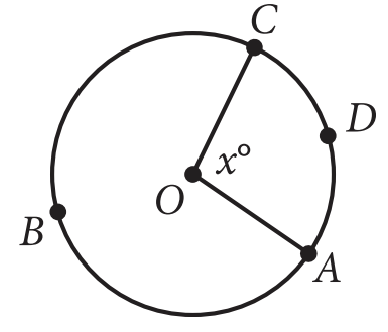
\includegraphics[width=0.52\linewidth]{23.png}
\end{center}

The circle above has center $O$, the length of arc $\wideparen{ADC}$ is $5\pi$, and $x = 100$. What is the length of arc $\wideparen{ABC}$?
\begin{itemize}
    \item[\textbf{A.}] $9\pi$
    \item[\textbf{B.}] $13\pi$
    \item[\textbf{C.}] $18\pi$
    \item[\textbf{D.}] $\dfrac{13\pi}{2}$
\end{itemize}
\end{frame}
\begin{frame}{Answer: The circle above has center O, the length of arc ADC is 5 , and x = 100.…}
\textit{Strategy:} Standard form $(x-h)^2+(y-k)^2=r^2$ reveals center and radius.

\textbf{Correct Answer:} \( \boxed{B} \)

\end{frame}
\begin{frame}{Question: The graph of x2 + x + y2 + y = 199/2 in the xy-plane is a circle. What i…}
The graph of $x^2 + x + y^2 + y = \dfrac{199}{2}$ in the $xy$-plane is a circle. What is the length of the circle’s radius?
\end{frame}
\begin{frame}{Answer: The graph of x2 + x + y2 + y = 199/2 in the xy-plane is a circle. What i…}
\textit{Strategy:} Complete the square on both $x$ and $y$.

\textbf{Solution:}
\[ \boxed{10} \]
\textbf{Correct Answer:} \( \boxed{10} \)

\end{frame}
\begin{frame}{Question: x2 + 20x + y2 + 16y = -20}
\[
x^2 + 20x + y^2 + 16y = -20
\]

The equation above defines a circle in the $xy$-plane. What are the coordinates of the center of the circle?
\begin{itemize}
    \item[\textbf{A.}] $(-20, -16)$
    \item[\textbf{B.}] $(-10, -8)$
    \item[\textbf{C.}] $(10, 8)$
    \item[\textbf{D.}] $(20, 16)$
\end{itemize}
\end{frame}
\begin{frame}{Answer: x2 + 20x + y2 + 16y = -20}
\textit{Strategy:} Distance from center to point equals radius.

\textbf{Correct Answer:} \( \boxed{B} \)

\end{frame}
\begin{frame}{Question: Point O is the center of the circle above, and the measure of OAB is 30°…}
\begin{center}
    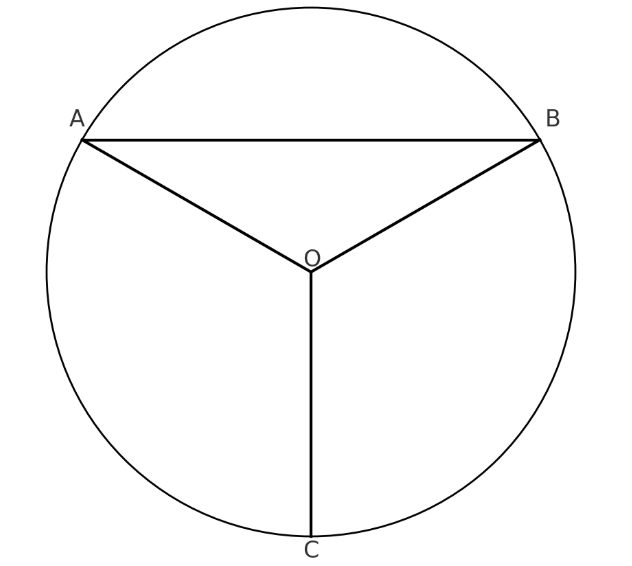
\includegraphics[width=0.55\linewidth]{24.png}
\end{center}

Point $O$ is the center of the circle above, and the measure of $\angle OAB$ is $30^\circ$. If the length of $\overline{OC}$ is $18$, what is the length of arc $\wideparen{AB}$?
\begin{itemize}
    \item[\textbf{A.}] $9\pi$
    \item[\textbf{B.}] $12\pi$
    \item[\textbf{C.}] $15\pi$
    \item[\textbf{D.}] $18\pi$
\end{itemize}
\end{frame}
\begin{frame}{Answer: Point O is the center of the circle above, and the measure of OAB is 30°…}
\textit{Strategy:} Tangent line is perpendicular to the radius at the point of tangency.

\textbf{Correct Answer:} \( \boxed{B} \)

\end{frame}
\begin{frame}{Question: A circle in the xy-plane has a diameter with endpoints (2, 4) and (2, 14…}
A circle in the $xy$-plane has a diameter with endpoints $(2, 4)$ and $(2, 14)$. An equation of this circle is $(x - 2)^2 + (y - 9)^2 = r^2$, where $r$ is a positive constant. What is the value of $r$?
\end{frame}
\begin{frame}{Answer: A circle in the xy-plane has a diameter with endpoints (2, 4) and (2, 14…}
\textit{Strategy:} Substitute the point into the circle equation to solve for $r$ or $k$.

\textbf{Solution:}
\[ \boxed{5} \]
\textbf{Correct Answer:} \( \boxed{5} \)

\end{frame}
\begin{frame}{Question: Circle A in the xy-plane has the equation (x + 5)2 + (y - 5)2 = 4. Circl…}
Circle $A$ in the $xy$-plane has the equation $(x + 5)^2 + (y - 5)^2 = 4$. Circle $B$ has the same center as circle $A$. The radius of circle $B$ is two times the radius of circle $A$. The equation defining circle $B$ in the $xy$-plane is $(x + 5)^2 + (y - 5)^2 = k$, where $k$ is a constant. What is the value of $k$?
\end{frame}
\begin{frame}{Answer: Circle A in the xy-plane has the equation (x + 5)2 + (y - 5)2 = 4. Circl…}
\textit{Strategy:} Shift $y$ by $k$ in the equation to move the center vertically.

\textbf{Solution:}
\[ \boxed{16} \]
\textbf{Correct Answer:} \( \boxed{16} \)

\end{frame}
\begin{frame}{Question: What is the diameter of the circle in the xy-plane with equation (x - 5)…}
What is the diameter of the circle in the $xy$-plane with equation $(x - 5)^2 + (y - 3)^2 = 16$?
\begin{itemize}
    \item[\textbf{A.}] $4$
    \item[\textbf{B.}] $8$
    \item[\textbf{C.}] $16$
    \item[\textbf{D.}] $32$
\end{itemize}
\end{frame}
\begin{frame}{Answer: What is the diameter of the circle in the xy-plane with equation (x - 5)…}
\textit{Strategy:} Expand and match coefficients after completing the square.

\textbf{Correct Answer:} \( \boxed{B} \)

\end{frame}
\begin{frame}{Question: Point O is the center of a circle. The measure of arc RS on this circle …}
Point $O$ is the center of a circle. The measure of arc $\overarc{RS}$ on this circle is $100^\circ$. What is the measure, in degrees, of its associated angle $\angle ROS$?
\end{frame}
\begin{frame}{Answer: Point O is the center of a circle. The measure of arc RS on this circle …}
\textit{Strategy:} Two circles: compare centers and radii for intersection.

\textbf{Solution:}
\[ \boxed{100} \]
\textbf{Correct Answer:} \( \boxed{100} \)

\end{frame}
\begin{frame}{Question: The equation (x + 6)2 + (y + 3)2 = 121 defines a circle in the xy-plane.…}
The equation $(x + 6)^2 + (y + 3)^2 = 121$ defines a circle in the $xy$-plane. What is the radius of the circle?
\end{frame}
\begin{frame}{Answer: The equation (x + 6)2 + (y + 3)2 = 121 defines a circle in the xy-plane.…}
\textit{Strategy:} Arc length $=\dfrac{\theta}{360^\circ}\cdot 2\pi r$.

\textbf{Solution:}
\[ \boxed{11} \]
\textbf{Correct Answer:} \( \boxed{11} \)

\end{frame}
\begin{frame}{Question: A circle in the xy-plane has its center at (-4, -6). Line k is tangent t…}
A circle in the $xy$-plane has its center at $(-4, -6)$. Line $k$ is tangent to this circle at the point $(-7, -7)$. What is the slope of line $k$?
\begin{itemize}
    \item[\textbf{A.}] $-3$
    \item[\textbf{B.}] $-\dfrac{1}{3}$
    \item[\textbf{C.}] $\dfrac{1}{3}$
    \item[\textbf{D.}] $3$
\end{itemize}
\end{frame}
\begin{frame}{Answer: A circle in the xy-plane has its center at (-4, -6). Line k is tangent t…}
\textit{Strategy:} Sector area $=\dfrac{\theta}{360^\circ}\cdot \pi r^2$.

\textbf{Correct Answer:} \( \boxed{A} \)

\end{frame}
\begin{frame}{Question: A circle has center O, and points R and S lie on the circle. In triangle…}
A circle has center $O$, and points $R$ and $S$ lie on the circle. In triangle $ORS$, the measure of $\angle ROS$ is $88^\circ$. What is the measure of $\angle RSO$, in degrees? (Disregard the degree symbol when entering your answer.)
\end{frame}
\begin{frame}{Answer: A circle has center O, and points R and S lie on the circle. In triangle…}
\textit{Strategy:} Inscribed angle relates to intercepted arc.

\textbf{Solution:}
\[ \boxed{46} \]
\textbf{Correct Answer:} \( \boxed{46} \)

\end{frame}
\begin{frame}{Question: In the xy-plane, the graph of 2x2 - 6x + 2y2 + 2y = 45 is a circle. What…}
In the $xy$-plane, the graph of $2x^2 - 6x + 2y^2 + 2y = 45$ is a circle. What is the radius of the circle?
\begin{itemize}
    \item[\textbf{A.}] $5$
    \item[\textbf{B.}] $6.5$
    \item[\textbf{C.}] $\sqrt{40}$
    \item[\textbf{D.}] $\sqrt{50}$
\end{itemize}
\end{frame}
\begin{frame}{Answer: In the xy-plane, the graph of 2x2 - 6x + 2y2 + 2y = 45 is a circle. What…}
\textit{Strategy:} Use the distance formula for chord length or radius.

\textbf{Correct Answer:} \( \boxed{A} \)

\end{frame}
\begin{frame}{Question: The equation x2 + (y - 1)2 = 49 represents circle A. Circle B is obtaine…}
The equation $x^2 + (y - 1)^2 = 49$ represents circle $A$. Circle $B$ is obtained by shifting circle $A$ down 2 units in the $xy$-plane. Which of the following equations represents circle $B$?
\begin{itemize}
    \item[\textbf{A.}] $(x + 2)^2 + (y - 1)^2 = 49$
    \item[\textbf{B.}] $x^2 + (y - 3)^2 = 49$
    \item[\textbf{C.}] $(x - 2)^2 + (y - 1)^2 = 49$
    \item[\textbf{D.}] $x^2 + (y + 1)^2 = 49$
\end{itemize}
\end{frame}
\begin{frame}{Answer: The equation x2 + (y - 1)2 = 49 represents circle A. Circle B is obtaine…}
\textit{Strategy:} Perpendicular from center bisects a chord.

\textbf{Correct Answer:} \( \boxed{D} \)

\end{frame}
\begin{frame}{Question: A circle has center O, and points A and B lie on the circle. The measure…}
A circle has center $O$, and points $A$ and $B$ lie on the circle. The measure of arc $\overarc{AB}$ is $45^\circ$ and the length of arc $\overarc{AB}$ is $3$ inches. What is the circumference, in inches, of the circle?
\begin{itemize}
    \item[\textbf{A.}] $3$
    \item[\textbf{B.}] $6$
    \item[\textbf{C.}] $9$
    \item[\textbf{D.}] $24$
\end{itemize}
\end{frame}
\begin{frame}{Answer: A circle has center O, and points A and B lie on the circle. The measure…}
\textit{Strategy:} System: substitute line into circle equation.

\textbf{Correct Answer:} \( \boxed{D} \)

\end{frame}
\begin{frame}{Question: Which of the following equations represents a circle in the xy-plane tha…}
Which of the following equations represents a circle in the $xy$-plane that intersects the $y$-axis at exactly one point?
\begin{itemize}
    \item[\textbf{A.}] $(x - 8)^2 + (y - 8)^2 = 16$
    \item[\textbf{B.}] $(x - 8)^2 + (y - 4)^2 = 16$
    \item[\textbf{C.}] $(x - 4)^2 + (y - 9)^2 = 16$
    \item[\textbf{D.}] $x^2 + (y - 9)^2 = 16$
\end{itemize}
\end{frame}
\begin{frame}{Answer: Which of the following equations represents a circle in the xy-plane tha…}
\textit{Strategy:} Graph the center and radius; read intercepts from symmetry.

\textbf{Correct Answer:} \( \boxed{C} \)

\end{frame}
\begin{frame}{Question: In the xy-plane, the graph of the equation above is a circle. Point P is…}
In the $xy$-plane, the graph of the equation above is a circle. Point $P$ is on the circle and has coordinates $(10, -5)$. If $\overline{PQ}$ is a diameter of the circle, what are the coordinates of point $Q$?

\[
(x - 6)^2 + (y + 5)^2 = 16
\]
\begin{itemize}
    \item[\textbf{A.}] $(2, -5)$
    \item[\textbf{B.}] $(6, -1)$
    \item[\textbf{C.}] $(6, -5)$
    \item[\textbf{D.}] $(6, -9)$
\end{itemize}
\end{frame}
\begin{frame}{Answer: In the xy-plane, the graph of the equation above is a circle. Point P is…}
\textit{Strategy:} Angle in semicircle or central vs. inscribed angle relationship.

\textbf{Correct Answer:} \( \boxed{A} \)

\end{frame}
\begin{frame}{Question: A circle in the xy-plane has its center at (-5, 2) and has a radius of 9…}
A circle in the $xy$-plane has its center at $(-5, 2)$ and has a radius of $9$. An equation of this circle is $x^2 + y^2 + ax + by + c = 0$, where $a$, $b$, and $c$ are constants. What is the value of $c$?
\end{frame}
\begin{frame}{Answer: A circle in the xy-plane has its center at (-5, 2) and has a radius of 9…}
\textit{Strategy:} Reflect over center to find symmetric point on the circle.

\textbf{Solution:}
\[ \boxed{-52} \]
\textbf{Correct Answer:} \( \boxed{-52} \)

\end{frame}
\begin{frame}{Question: The equation x2 + (y - 2)2 = 36 represents circle A. Circle B is obtaine…}
The equation $x^2 + (y - 2)^2 = 36$ represents circle $A$. Circle $B$ is obtained by shifting circle $A$ down $4$ units in the $xy$-plane. Which of the following equations represents circle $B$?
\begin{itemize}
    \item[\textbf{A.}] $x^2 + (y - 6)^2 = 36$
    \item[\textbf{B.}] $x^2 + (y + 2)^2 = 36$
    \item[\textbf{C.}] $(x - 4)^2 + (y - 2)^2 = 36$
    \item[\textbf{D.}] $(x + 4)^2 + (y - 2)^2 = 36$
\end{itemize}
\end{frame}
\begin{frame}{Answer: The equation x2 + (y - 2)2 = 36 represents circle A. Circle B is obtaine…}
\textit{Strategy:} Slope of tangent is negative reciprocal of radius slope.

\textbf{Correct Answer:} \( \boxed{B} \)

\end{frame}
\begin{frame}{Question: Points A and B lie on a circle with radius 1, and arc AB has length /3. …}
Points $A$ and $B$ lie on a circle with radius $1$, and arc $\overarc{AB}$ has length $\dfrac{\pi}{3}$. What fraction of the circumference of the circle is the length of arc $\overarc{AB}$?
\end{frame}
\begin{frame}{Answer: Points A and B lie on a circle with radius 1, and arc AB has length /3. …}
\textit{Strategy:} Difference of areas of two circles with radii $R$ and $r$.

\textbf{Solution:}
\[ \boxed{1/6} \]
\textbf{Correct Answer:} \( \boxed{1/6} \)

\end{frame}
\begin{frame}{Question: A circle in the xy-plane has equation (x + 3)2 + (y - 1)2 = 25. Which of…}
A circle in the $xy$-plane has equation $(x + 3)^2 + (y - 1)^2 = 25$. Which of the following points does NOT lie in the interior of the circle?
\begin{itemize}
    \item[\textbf{A.}] $(-7, 3)$
    \item[\textbf{B.}] $(-3, 1)$
    \item[\textbf{C.}] $(0, 0)$
    \item[\textbf{D.}] $(3, 2)$
\end{itemize}
\end{frame}
\begin{frame}{Answer: A circle in the xy-plane has equation (x + 3)2 + (y - 1)2 = 25. Which of…}
\textit{Strategy:} Apply vertical/horizontal shift to center coordinates.

\textbf{Correct Answer:} \( \boxed{D} \)

\end{frame}

\begin{frame}{}
    \begin{tikzpicture}[remember picture, overlay]
        \shade[top color=novelPurple!40, bottom color=white]
            (current page.north west) rectangle (current page.south east);
        \fill[white, opacity=0.15] (current page.center) circle (5cm);
        \foreach \x in {1,2,3,4,5} {
            \fill[novelPurple, opacity=0.12] (rand*10-5, rand*7-3.5) circle (0.1+\x*0.05);
        }
    \end{tikzpicture}
    \centering
    \vspace{5em}
    {\Huge \textbf{\textcolor{novelPurple}{Thank You!}}} \\[1em]
    {\large \textcolor{gray}{We appreciate your time and focus.}} \\[3em]
    {\LARGE \textbf{\textcolor{novelPurple}{\textsf{Novel Prep}}}}
    \vfill
\end{frame}

\end{document}
